\section{Experimental evaluation}\label{sec:experiments}

The evaluation addresses four questions. Native runs link requests and rule writes to changes in resource state. Comparisons on identical inputs identify where global constraints yield a determinate verdict. Evidence ablations and deliberately incorrect assumptions test which observations support each conclusion. We measure the cost of online collection separately from that of offline analysis.

\begin{itemize}
\item \textbf{RQ1. Execution effects.} Can the method distinguish a request that reaches application processing, one that produces a successful action, and one that establishes new admission?
\item \textbf{RQ2. Global constraints.} When multiple source assignments are possible, under what conditions does a global query yield an additional determinate verdict?
\item \textbf{RQ3. Reliability.} Do the implemented queries agree with the model semantics, and how do missing observations or incorrect assumptions change their verdicts?
\item \textbf{RQ4. Cost.} How much control traffic does a legitimate admission exchange generate? How does enabling collection affect knock latency, application access latency, object goodput and the amount of data written to disk? How long do the solver and the complete offline invocation take?
\end{itemize}

\subsection{Experimental design}\label{sec:design}\label{sec:setup}

We use three sources of evidence. Native records test whether the two levels of attribution can be distinguished on the actual execution path. Controlled model inputs isolate the effects of candidate structure, query semantics and model assumptions. Archived traces show how gaps in the evidence constrain a verdict. To assess the contribution of evidence, we hold the run and target fixed and vary what a method can observe. To compare solvers, we fix both the candidate graph and the observation conditions (Fig.~\ref{fig:4}). Online collection and offline analysis have separate cost experiments.

The \href{https://github.com/B1ueD0g/opennhp-admission-attribution-artifact}{GitHub artifact repository} contains the offline verification code and both sealed synthetic suites. The data availability statement describes the scope of the archived records.

\begin{figure*}[t]
\centering
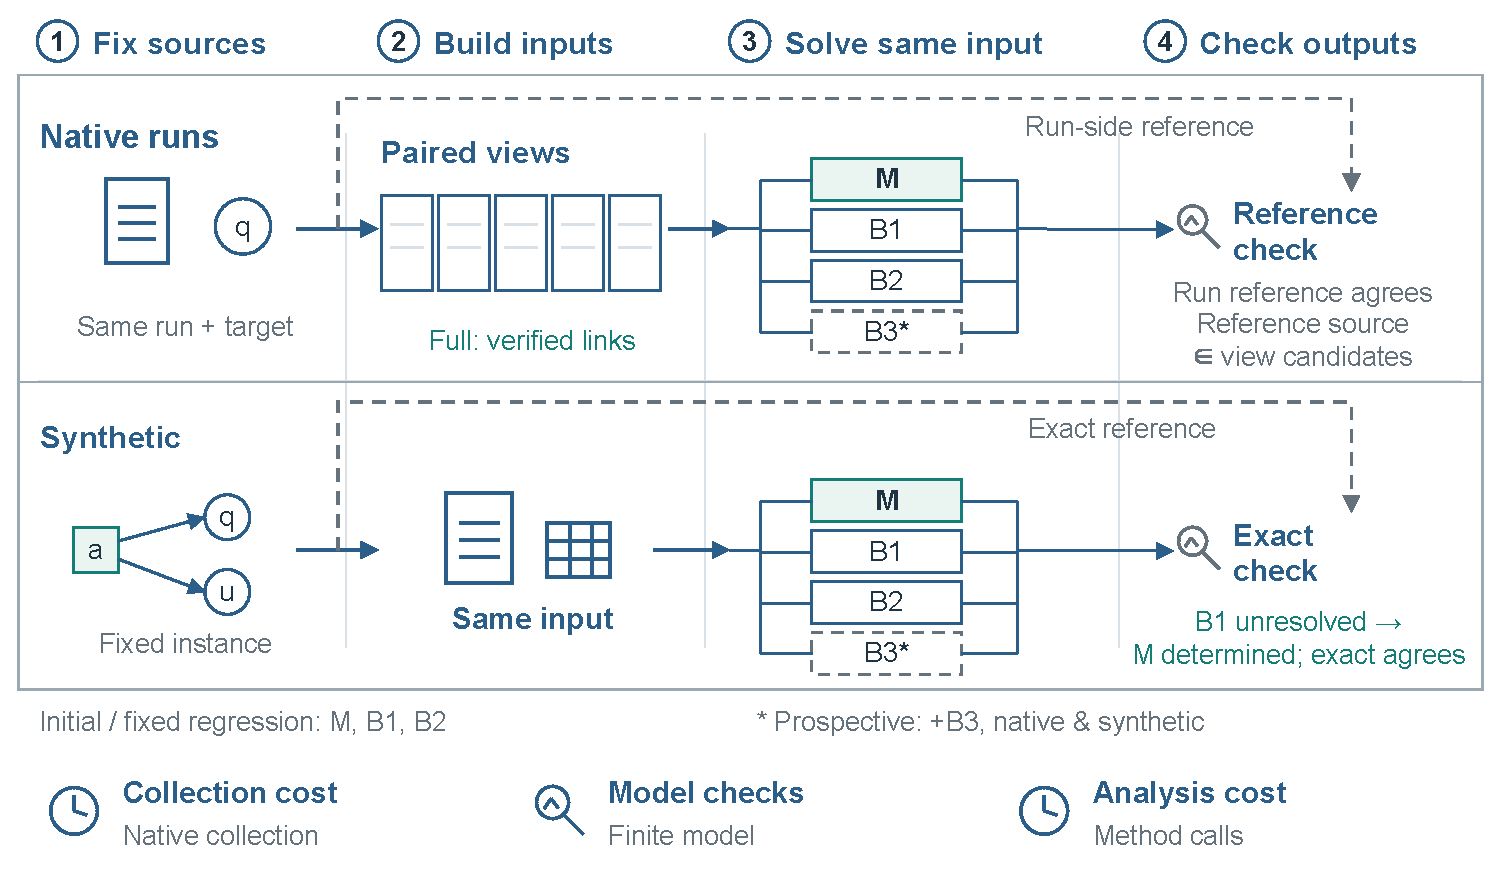
\includegraphics[width=\textwidth]{fig4.pdf}
\caption{Paired evaluation on native runs and synthetic instances. The columns show the source, input construction, method comparison, and output check. For native runs, verdicts from paired views of the same run and target are checked against the run-side reference. For synthetic instances, all methods receive the same input, and their verdicts are checked against exact enumeration. B3 participates in the follow-up native and prospective synthetic comparisons.}
\label{fig:4}
\end{figure*}

Table~\ref{tab:3} gives the unit, size and purpose of each cohort. We report inclusion separately for each cohort. A single run can support several target queries and paired views, and multiple methods can analyze the same input.

\paragraph{Native environment and scenarios.}
We used an AArch64 Lima VM with Alpine 3.23.3, Linux 6.18.7-0-virt, and Go 1.26.4 (CGO enabled). The tested OpenNHP revision was \nolinkurl{40e6b2a9e14d452629fa6af255fccbd37bca9807}~\citep{r42}. A virtual Ethernet pair (veth) connected the Agent and server-side namespaces. Neither namespace had a default route.

The Agent called the one-shot Knock API. The Server used the \texttt{example} plugin built from \texttt{basic}. The access controller (AC) installed rules using iptables and ipset. The protected service listened on TCP port 8080 with access denied by default. The HTTP management interface was disabled. Each window started with newly created namespaces, processes, rules and services.

The initial scenarios covered first admission (C1), a fresh request after expiry (C2), successive writes from three Agents (C3), and backend authentication after entry into application processing (C4). The formal follow-up comprised three blocks. Each block included one window for each of five scenarios: empty input (C0), C2, C4, and two Agents acting either serially (C5S) or synchronously (C5P). In C5S, the second Agent was released after the first handler completed. In C5P, both Agents shared a release barrier. A window could contain several requests, with paired views constructed for each target query.

\begin{table*}[t]
\centering
\caption{Evaluation cohorts, units of observation and comparison conditions.}
\label{tab:3}
\small
\begin{tabularx}{\textwidth}{@{}>{\raggedright\arraybackslash}p{.17\textwidth}>{\raggedright\arraybackslash}p{.29\textwidth}>{\raggedright\arraybackslash}Xl@{}}
\toprule
Cohort & Size and unit & Comparison or purpose & Question \\
\midrule
Initial native runs & 12 windows executed, 6 eligible, 10 target queries & Paired views of the same run for reconstructing action and admission evidence & RQ1, RQ3 \\
Formal native runs & 15 windows executed, 12 eligible, 18 queries including 3 empty inputs & Fixed scenarios and build for comparison across methods and observation conditions & RQ1--RQ3 \\
Engineering pilot & 4 windows, 6 queries, including 1 synchronous window with 2 queries & Separately reported witness of interchangeable source assignments & RQ2 \\
C4 repeat & 3 windows, 3 queries, separate from the formal cohort & Restore the 10-s collection wait and check for completion records & RQ1, RQ3 \\
\addlinespace
Fixed regression suite & 24 development and 24 sealed instances, rerun after corrections & Same-input baselines, diagnostic variants and equivalent encodings & RQ2, RQ3 \\
Prospective sealed suite & 24 instances in 4 groups of 6, 96 first-round method calls & Four methods on fixed inputs, reference labels released after the first round & RQ2, RQ3 \\
Model and assumption checks & 26,880 inputs and 4 additional types of target-absent input & Independent enumeration, 6 types of incorrect assumptions and 7 lifecycle ablations & RQ3 \\
Archived diagnostics & 6 KNK scenarios with 3 runs each, 16 incomplete inputs, 312 V2 records & Evidence gaps and authorization assessed within each source's coverage & RQ3 \\
\addlinespace
Online collection cost & 20 blocks $\times$ 4 conditions, 80 windows & Same instrumented build, varying event recording and packet capture & RQ4 \\
Offline analysis cost & 24 instances $\times$ 4 methods $\times$ 5 blocks, 480 calls & Same base inputs, fresh process on every call & RQ4 \\
\bottomrule
\end{tabularx}
\end{table*}

The initial query count excludes the preparatory C2 request. The formal cohort contains 15 queries on actual requests and three empty-input controls. Archived datasets can draw on the same historical runs, so their counts do not form an independent sample total.

\paragraph{Observation and inclusion.}
We used tcpdump 4.99.5 and libpcap 1.10.7 to capture traffic on veth and loopback (lo). Process events covered receipt, application handling, plugin callbacks, AOP, rule writes and ART. Process-start identifiers and process-local monotonic sequence numbers distinguished events. We verified links across processes using transaction identifiers, peer identities in both directions, and endpoints. For each cohort, we verified the build, loaded objects, configuration, processes and rule writer, and reconciled captures against process events. The initial cohort required the prespecified post-state as one of its inclusion criteria. For the follow-up, inclusion required complete capture, execution of the intended scenario, capacity support, and consistency of the explicit links in the reference records. We recorded the measured post-state separately, whether the probe returned no HTTP response (coded 000) or HTTP~200. C0 also had to satisfy the empty-input control. Appendix~B gives the window-level inclusion decisions.

We constructed five observation views of each run to evaluate source constraints (Section~\ref{sec:target-action}) and resource conditions (Section~\ref{sec:new-admission}). The full view retains the explicit request link. The restricted view hides that link and retains the remaining evidence. Three further views each withdraw one condition from the restricted view: completeness of request records, completeness of action records, or evidence of an initially empty rule set (Fig.~\ref{fig:5}). Withdrawing a completeness assertion retains all recorded events and admits explanations involving missing events. Withdrawing the empty pre-state changes what can be inferred about the resource transition.

\begin{figure*}[t]
\centering
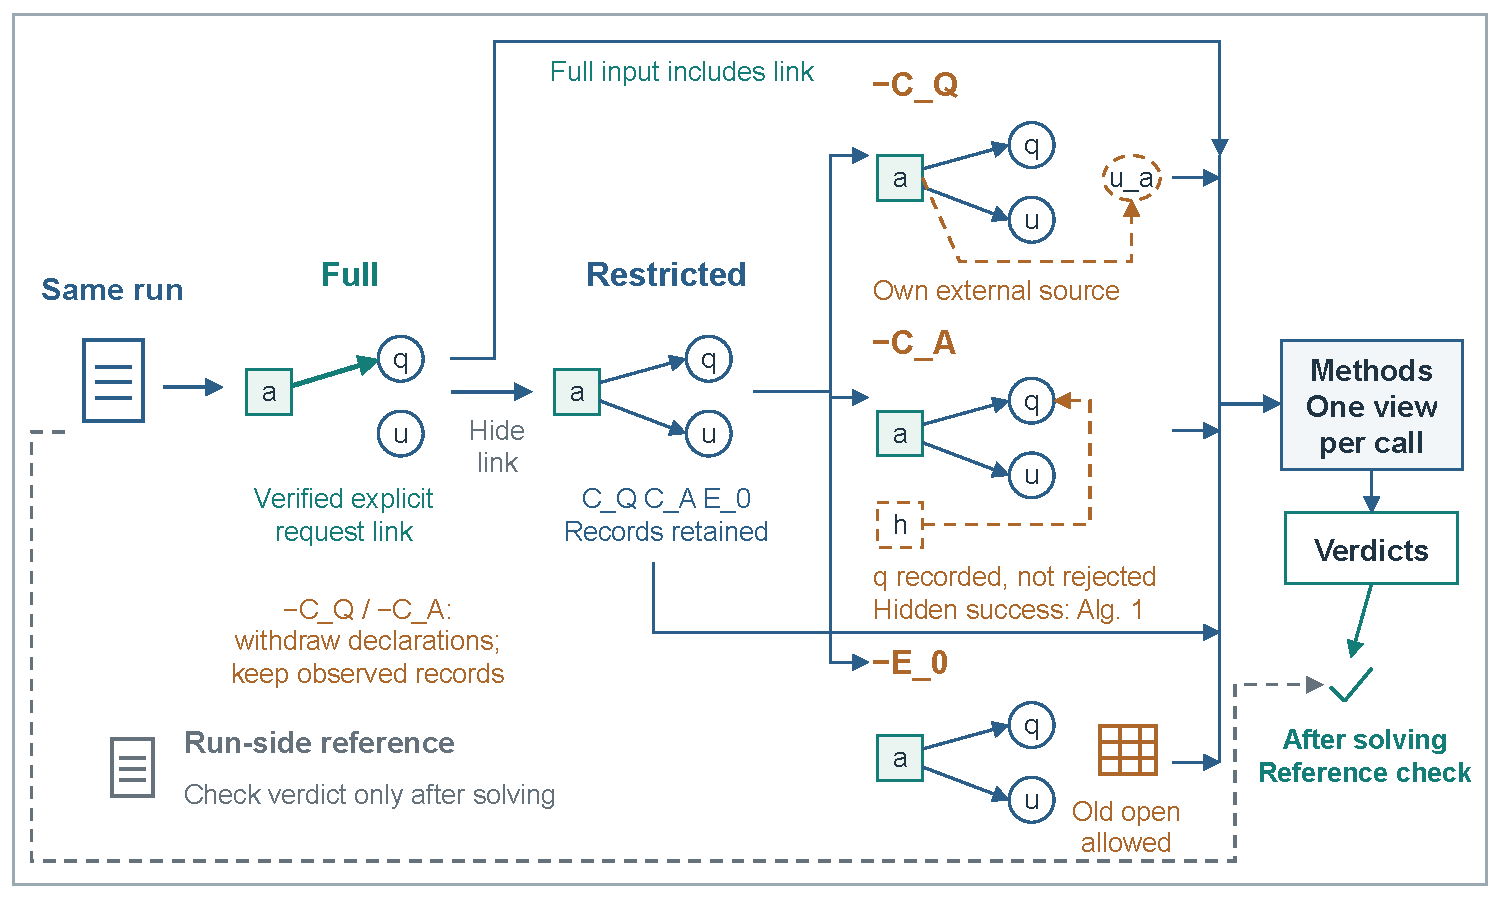
\includegraphics[width=\textwidth]{fig5.pdf}
\caption{Construction of paired views from a single run. Full retains the verified request link. Restricted hides it. Each ablation starts from Restricted and retains existing records. Each solver call receives one view, and the reference verdict is consulted after the call.}
\label{fig:5}
\end{figure*}

In the restricted view, a candidate request had to target the same resource and be handled by the same NHP-Server process. The AOP for the bundle had to be created within that request's processing interval. All methods received the same input for a given view. After solving, we checked both the processing state and the execution effect against the run-side reference. That reference retained the explicit request link hidden from the restricted view, together with transactions, peer identities, endpoints, rule readbacks and probe records.

Four observation sources support these views (Fig.~\ref{fig:6}). Captures on veth and lo cover control and application traffic. Process events link requests to execution. Rule readbacks establish rule state, and independent probes check fresh connections and service health. A SYN records an attempted connection. A complete handshake identifies a fresh TCP connection. The connection and unique request identifier associate the GET with its HTTP~200 response~\citep{r43,r44}.

\begin{figure*}[t]
\centering
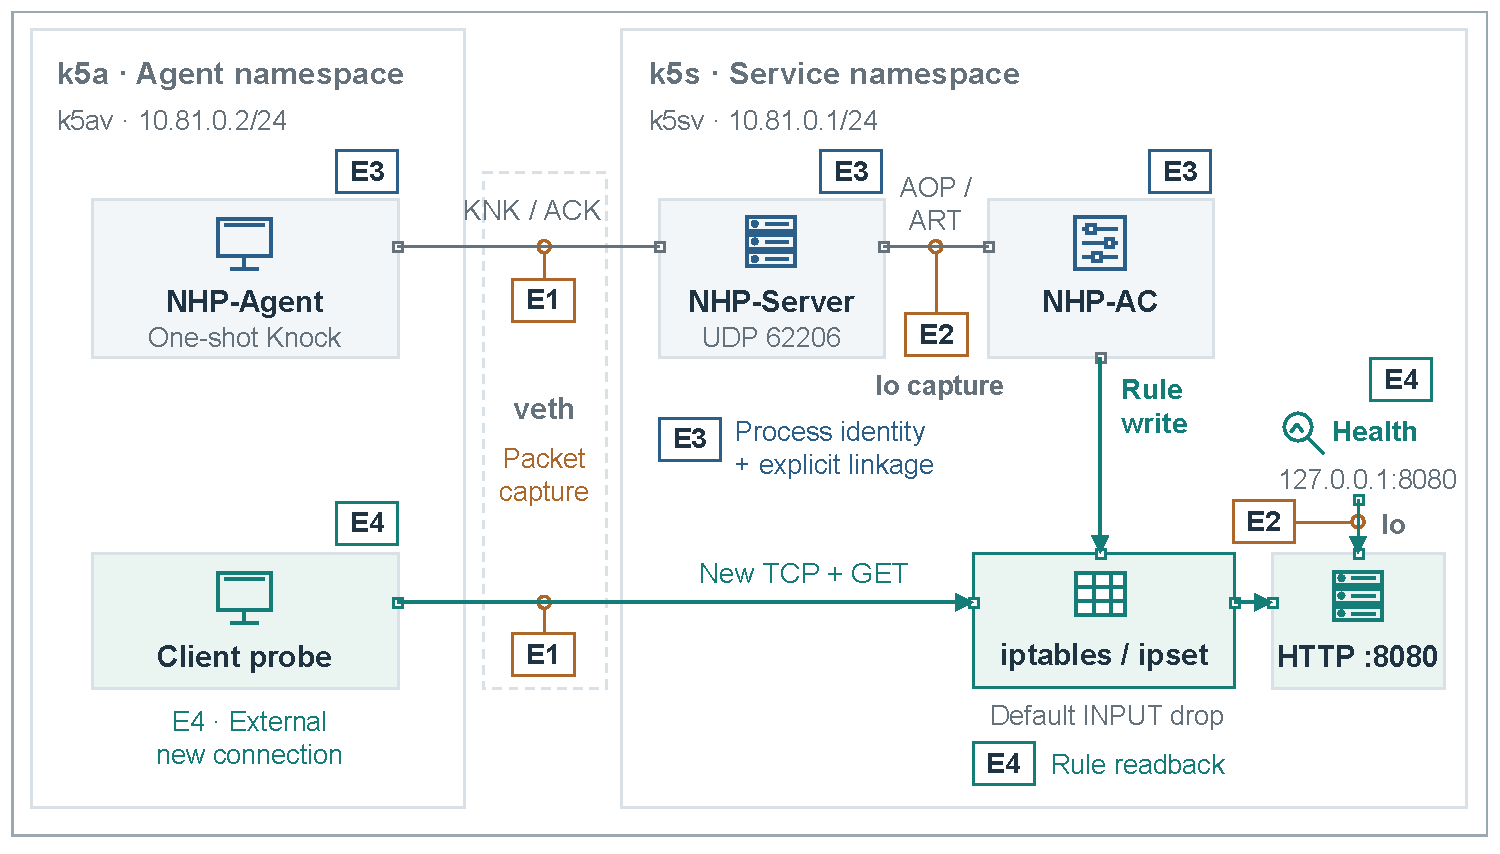
\includegraphics[width=\textwidth]{fig6.pdf}
\caption{Observation points on the native KNK path. E1 captures veth traffic and E2 captures loopback traffic, including health checks. E3 records process events and explicit links. E4 supplies rule readbacks and active probes. Gray lines denote connectivity and teal arrows denote writes or access.}
\label{fig:6}
\end{figure*}

Successful access required a fresh handshake, a GET carrying the unique identifier, and its matching HTTP~200 response. For unsuccessful access, we required an external SYN without a completed handshake and an independent health check. In C2, the configured \texttt{OpenTime} was 3~s, while the AC command used 8~s. After 9.2~s, the rule readback was empty, a new external connection received no HTTP response, and the service remained healthy. Together these observations confirmed expiry.

\paragraph{Same-input baselines.}
All methods received the same requests, candidate relations and observation conditions. The global method (M) and local propagation (B1) share input validation and output rules. Under unit capacity, B1 assigns each bundle with a single candidate source and deducts the capacity consumed at that source. It also checks whether the whole graph admits a matching. Successful bundles assigned to the target give a lower bound on its number of successful actions. Remaining candidates and any permissible unrecorded action give an upper bound. M also modifies edges incident to the target and retests feasibility. This tests explanations in which the target succeeds and explanations in which it has no success. An unrecorded success must also fit the available capacity. Exact enumeration (B2) traverses compatible explanations, while minimum-cost flow (B3) solves the same finite model. Both check the bounds on the target's success count, possible unrecorded actions and competing writes. A separate control retains the request processing state and authorization rule but uses only post-state HTTP reachability to judge the effect.

The initial native and fixed regression cohorts compare M, B1 and B2. B3 joins the follow-up native and prospective synthetic comparisons. Each method returns run status, request processing state, execution effect and authorization conformance. For the exact methods we also check the applicable \emph{must} and \emph{may} values. In the follow-up, we count a gain only if B1 is unresolved, M is determinate and both exact baselines agree with M. Native gains must also agree with the run-side reference, and the source identified by that reference must belong to the restricted view's candidate set. Native replay of recorded inputs and the prospective synthetic comparisons had a 10-s limit per call. B2 also had a limit of 100,000 compatible explanations. Native inputs contained at most eight requests and eight action bundles. We report conflicts, invalid inputs and budget overruns separately.

\paragraph{Controlled model inputs and archived records.}
Model validation and regression used 24 development and 24 sealed base instances, together with equivalent encodings. Inputs and code were frozen before the first evaluation. After correcting input validation and query applicability, we reran the original suite. We report that rerun as regression evidence. For the prospective comparison, we generated and sealed 24 further synthetic instances, six in each of four groups: capacity-determined outcomes, explanations with opposite outcomes, infeasible assignments, and missing observations. We checked their labeled candidate graphs for duplicates against 96 historical inputs. The same team generated and sealed the instances. It disclosed the reference labels after recording the first outputs from all four methods. The archival diagnostics use historical KNK runs, 16 incomplete inputs and 312 V2 records.

\paragraph{Reliability checks.}
The finite-domain check fixes one resource, one or two requests, and zero to two action bundles. The first request is the target. All seven lifecycle conditions are true and the authorization requirement is unresolved. For each bundle we consider every subset of requests as candidate sources, distinguishing singleton sets with and without an explicit link. Action outcomes range over success, failure and unknown. Request states range over entry into application processing, rejection and unknown. We vary request-record completeness, action-record completeness and the capacity constraint over all on/off combinations. A separately implemented reference enumerates assignments, unknown outcomes and permissible unrecorded actions. Equivalent encodings and fresh-process replay test output stability. Observation ablations, incorrect assumptions and inputs without a target test the verdict boundaries.

\paragraph{Online collection cost.}
On a dedicated VM, we independently enabled or disabled event recording (T) and packet capture on both interfaces (C). T0C0, T1C0, T0C1 and T1C1 use identical binaries, plugin and configuration. All four retain the instrumentation call sites, so the contrast measures the increment from enabling collection. The VM had two vCPUs and 4~GiB of memory. Capture requested a 16~MiB buffer per interface. We froze 20 randomized complete blocks, each with one window per condition, for 80 windows. Each window used a separate directory, rebuilt the namespaces, rules and processes, and cleared prior state. No retry replaced a sample. Four preflight windows are reported separately in Appendix~E. The reference for this lightly loaded, single-VM experiment is the same build with collection disabled.

Each window began with an empty rule set, a failed fresh external connection and a healthy service. We then issued one legitimate Knock and timed the API call on the process-local monotonic clock, excluding initialization waits and process exit. The client used fresh TCP connections to retrieve in-memory objects of 64~B, 64~KiB, and 1~MiB. The order of the two larger objects alternated across blocks. We disabled connection reuse and compression and checked status, length and SHA-256. Time to first byte is the elapsed time from the HTTP call to receipt of the first response byte. It includes connection establishment. We calculate object goodput as the number of verified response-body bits divided by the time from issuing the request to completing the body read. That interval includes hashing during the read. It therefore measures local short-object completion rate~\citep{r45}. API latency and packet round-trip time were recorded separately~\citep{r46}. For each contrast, we subtracted the reference value from the comparison value within each block, then took the median of the 20 paired differences. We computed descriptive 95\% percentile intervals from 10,000 block resamples without adjusting for multiple comparisons.

\paragraph{Offline analysis cost.}
A separate host-side experiment compared M, B1, B2 and B3 on the 24 prospective sealed instances. Five complete blocks were randomized in advance. Every block covered each instance--method pair and every call used a fresh process. The resulting 480 calls recorded solver time, preparation time and total process time separately.

\subsection{Results}\label{sec:results}
\subsubsection{Execution effects of native requests (RQ1)}\label{sec:rq1}

Three native contrasts test the two levels of attribution. C4 asks whether the evidence can rule out a successful action after a request reaches application processing. C3 separates action success from new admission when several requests write the same resource. C1 and C2 test the resource pre- and post-states needed to establish new admission. Six of the 12 initial windows qualified, yielding ten evaluation queries: one with no successful target action, six with action only and three with new admission (Tables~\ref{tab:4} and~\ref{tab:5}).

\begin{table*}[t]
\centering
\caption{Window inclusion and observed capacity in the initial native cohort. Request and action counts refer to eligible windows.}
\label{tab:4}
\small
\begin{tabularx}{\textwidth}{@{}Xrrrr@{}}
\toprule
Scenario & Planned and run & Eligible & Requests & AOP bundles \\
\midrule
C1: first admission & 3 & 2 & 2 & 2 \\
C2: fresh request after expiry & 3 & 1 & 2 & 2 \\
C3: three Agents & 3 & 2 & 6 & 6 \\
C4: backend authentication & 3 & 1 & 1 & 0 \\
\midrule
Total & 12 & 6 & 11 & 10 \\
\bottomrule
\end{tabularx}
\end{table*}

Including the preparatory request that established the earlier admission in C2, the eligible windows contained 11 requests and ten AOP bundles. One request produced no AOP. Excluding the preparatory request left ten target queries and nine AOP bundles for comparison. The implementation and configuration used one callback, one resource, one AC and a fixed target. These constraints supported an upper bound of one bundle per request, consistent with the observed counts.

Both first admission and admission after expiry require evidence that the resource was previously closed. In C1-r2 and C1-r3, the pre-write readback was empty. A fresh external connection received no HTTP response while the service remained healthy. After the write, the readback showed a rule from 10.81.0.2 to 10.81.0.1 for TCP port 8080, and a fresh connection succeeded. C2-r3 tests the same transition after an earlier rule expired (Fig.~\ref{fig:7}).

\begin{figure*}[t]
\centering
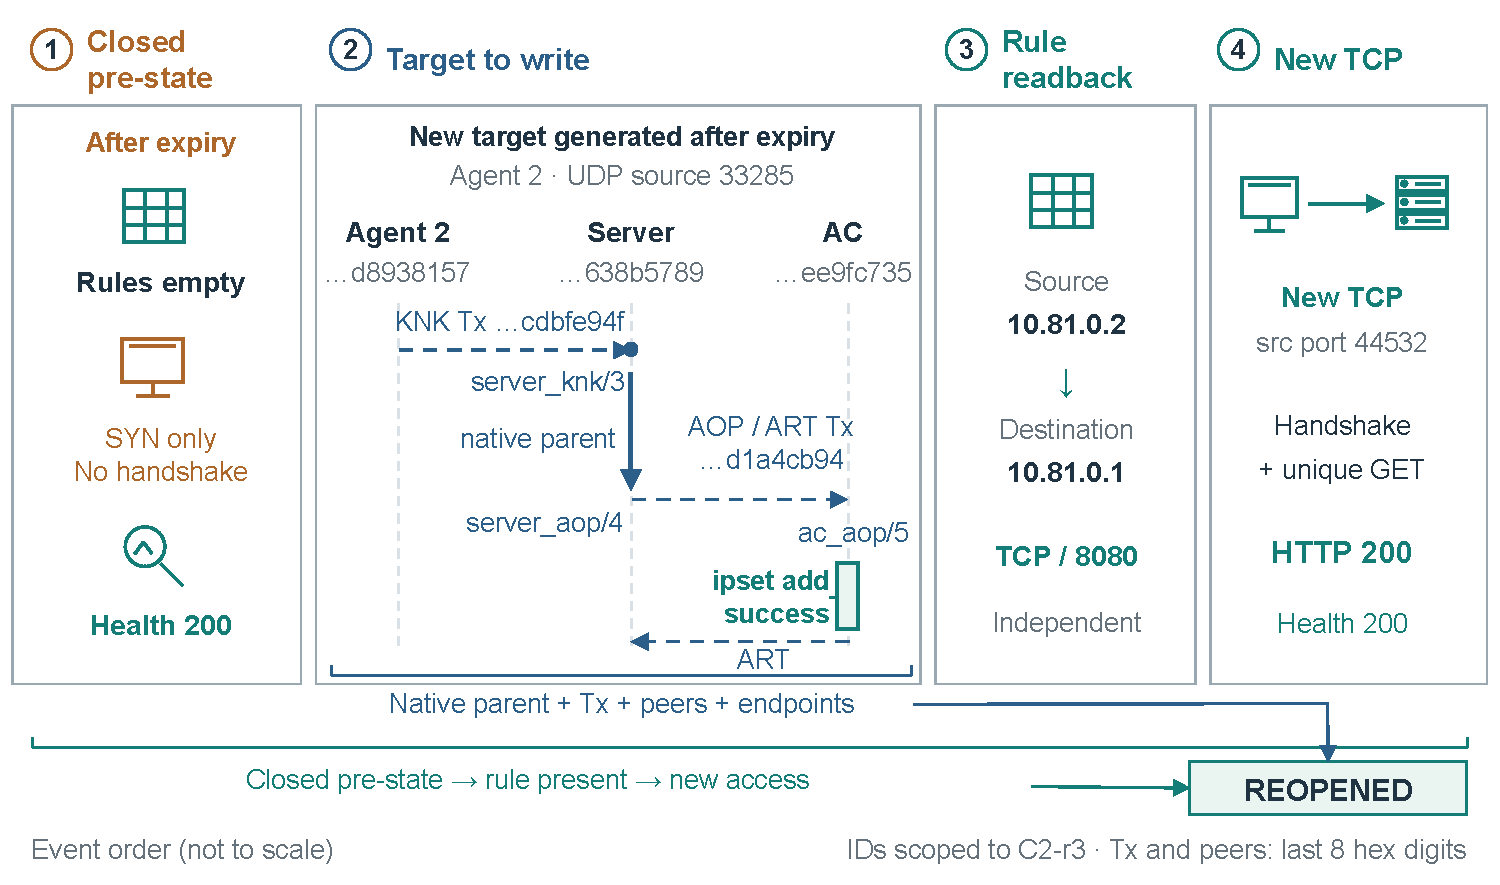
\includegraphics[width=\textwidth]{fig7.pdf}
\caption{Evidence for new admission in C2-r3. The four stages establish the pre-state, link the target to the write, independently read back the rule and verify access over fresh TCP. Transaction and peer identifiers show their last eight characters. Message spacing indicates order only.}
\label{fig:7}
\end{figure*}

The first stage in Fig.~\ref{fig:7} rules out continuing access from the preparatory request. After expiry, an independent readback found no rule. The external probe produced a SYN without a complete handshake, while the service-side health probe returned HTTP~200. A different configured Agent then generated a fresh request. Process-local evidence linked the request to the AOP, and cross-process transactions, peer identities and endpoints linked that AOP to a successful AC write. An independent readback confirmed the target rule before the application probe. A marked GET on a new TCP connection then received HTTP~200. The request and action records were complete and excluded competing writes to the same resource. Under these conditions, the new admission was attributable to the target. Appendix~B indexes the full transaction identifiers and captures.

In each of the two C3 windows, three requests wrote the same resource. All six successful actions had identifiable sources, but an alternative write in each window could explain final reachability. Each query therefore yields action only. C4 separates application processing from successful execution. Backend authentication returned 52007. Complete records contained neither a target helper invocation nor an AOP. The rule set remained empty, a fresh external connection received no HTTP response, and the health probe returned HTTP~200. The verdict was no successful target action (Table~\ref{tab:5}).

\begin{table*}[t]
\centering
\caption{Processing evidence and execution effects in the initial native cohort.}
\label{tab:5}
\small
\begin{tabularx}{\textwidth}{@{}l r X p{.22\textwidth}@{}}
\toprule
Scenario & Queries & Evidence of processing and action & Execution effect \\
\midrule
C1 & 2 & Reached application processing, successful write, target rule and fresh connection & 2 new admissions \\
C2 & 1 & Fresh request after confirmed expiry, matched target write and readback & 1 new admission \\
C3 & 6 & Six successful actions with identifiable sources, competing writes in each window & 6 action only \\
C4 & 1 & Reached application processing, backend returned 52007, no helper or AOP & 1 with no successful target action \\
\bottomrule
\end{tabularx}
\end{table*}

M, B1 and B2 agreed with the run-side reference on all ten initial queries under both full and restricted views. The other six windows in the initial cohort failed checks on capture completion, service identity, or reconciliation of health probes. An empty-input control lacked health evidence. A separate control with instrumentation switched off showed connection failure before the knock, followed by HTTP~200 and a matching rule after the knock, with successful health probes at both times. Both controls were excluded from the initial full comparison.

The formal follow-up extended the comparison to empty inputs and serial and synchronous request pairs. All four methods agreed on the 18 restricted-view queries: three new admissions, 12 action only and three with no successful target action (Table~\ref{tab:6}). Fifteen queries concerned actual requests. Three were C0 empty-input controls. M yielded zero additional determinate verdicts over B1.

\begin{table*}[t]
\centering
\caption{Four-method comparison under the restricted view in the formal follow-up cohort.}
\label{tab:6}
\small
\begin{tabularx}{\textwidth}{@{}p{.24\textwidth}r r X r@{}}
\toprule
Scenario & Eligible windows & Queries & Effect assigned by all four methods & Gain over B1 (M) \\
\midrule
C0: empty input & 3 & 3 & No successful target action & 0 \\
C2: fresh request after expiry & 3 & 3 & New admission & 0 \\
C5S: serial & 3 & 6 & Action only & 0 \\
C5P: synchronous & 3 & 6 & Action only & 0 \\
\midrule
Total & 12 & 18 & 3 new admissions, 12 action only, 3 with no successful target action & 0 \\
\bottomrule
\end{tabularx}
\end{table*}

Twelve of the 15 scheduled windows qualified. In the three C0 windows, no target request occurred, the rule set stayed empty and the external connection failed while the service remained healthy. All three C2 windows confirmed new admission after expiry. In the three formal C4 windows, completion records were still missing when the collection wait expired. Three separate repeat runs reinstated the 10-s wait and obtained complete records. Both views yielded no successful target action in all three. Figure~\ref{fig:8}(a) reports the repeats separately. Appendix~B gives the evidence for each inclusion decision.

Across the two native cohorts, C4 distinguishes application processing from action success. C3 shows why a successful action can leave the source of admission unresolved, and C1 and C2 show what evidence establishes a new admission. The next comparison tests how the candidate structure affects methods that see the same input.
\subsubsection{Candidate structure and the gain from global inference (RQ2)}

Overlapping candidates can leave the target outcome unresolved after local propagation. A global query can add a verdict if capacity constraints resolve that outcome. Once explicit links were hidden in the ten initial queries, each of the nine action bundles still had a single candidate. In the 18 formal native queries, processing intervals did not overlap in serial windows. The three synchronous C5P windows (six queries) did contain overlapping candidates, but each window had a bundle with only one candidate. Propagating its assignment and the remaining capacities determined the other assignments (upper panel of Fig.~\ref{fig:3}). Consequently, M resolved no additional queries over B1 in either native cohort. Figure~\ref{fig:8} shows which formal windows qualified and how each query changed across observation views; the coverage tests are examined under RQ3.

\begin{figure*}[t]\centering
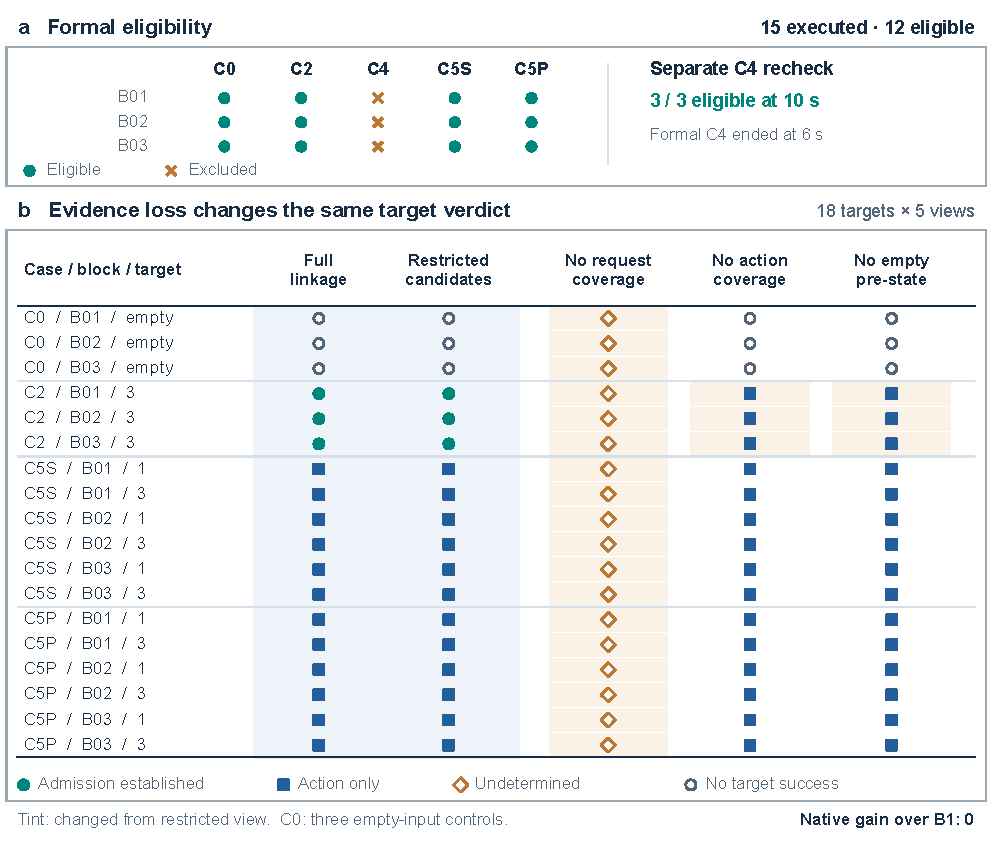
\includegraphics[width=\textwidth]{fig8.pdf}
\caption{Formal native windows and paired verdicts. (a) Twelve of 15 windows qualified; three independent C4 checks are shown separately. (b) Each row is one query, including three empty C0 inputs. The last three views remove request coverage, action coverage, or evidence of an initially empty rule set. Light amber marks changes from the restricted view.}\label{fig:8}
\end{figure*}

The four-window engineering pilot exhibited an exchangeable assignment structure (P-C5P; lower panel of Fig.~\ref{fig:3}). In one synchronous window, two successful bundles could each be assigned to either of two requests. B1 left both targets unresolved. M, B2, and B3 agreed with the run-side reference. In either feasible assignment, each target accounted for one successful action. Because both writes affected the same resource, neither could be credited individually with establishing admission. This mechanism check was independent of the formal cohort.

Global capacity constraints can thus settle whether a target succeeded even when local propagation cannot settle the assignment. On the 24 sealed fixed-regression instances, M resolved seven cases left open by B1: five as action only and two as admission established. M matched all four outputs of B2 on 24/24 instances. B1 matched all four on 17/24 instances (Table~\ref{tab:7}). Removing either request coverage or the unit-capacity constraint returned all seven to unresolved. Removing action coverage preserved successful-action attribution in all seven but removed the evidence for new admission in two.

\begin{table*}[t]\centering
\caption{Comparison on identical inputs from the fixed synthetic suite. Agreement requires a match on all four outputs.}\label{tab:7}
\small\begin{tabularx}{\textwidth}{@{}Xrrrrrr@{}}\toprule
Method & Agreement with B2 & Admission & Action only & No successful target action & Unresolved & Conflict\\\midrule
M: global queries & 24/24 & 3 & 8 & 7 & 3 & 3\\
B1: local propagation & 17/24 & 1 & 3 & 7 & 10 & 3\\
B2: exact enumeration & Reference & 3 & 8 & 7 & 3 & 3\\\bottomrule
\end{tabularx}\end{table*}

Two instances illustrate the distinction. In \texttt{sealed-09}, failed actions exhaust the capacity of two competing requests. Only the target can account for the successful bundle, and the resource observations also establish new admission. In \texttt{sealed-10}, the two successful bundles are exchangeable: every feasible assignment gives the target a successful write, but the competing write prevents attribution of admission. Capacity identifies the source of the successful write in the first instance. In the second, the target succeeds under either assignment even though the two writes remain exchangeable.

The prospective suite contained six instances in each of four structural groups. All six additional verdicts arose in the capacity-determined group (Fig.~\ref{fig:9}a). In three, failed actions exhausted competing capacity and the sole successful bundle, together with resource evidence, established admission for the target. In the other three, exchangeable successful writes established action only. All four methods agreed on execution effects for the remaining 18 instances (Fig.~\ref{fig:9}b). Across the initial 96 calls, M, B2 and B3 agreed on run status, processing status, effect, authorization mapping and the values of \textit{must} and \textit{may} where applicable. Their effects matched the sealed reference on 24/24 instances, compared with 18/24 for B1. Figure~\ref{fig:9}c distinguishes this cohort from fixed regression.

\begin{figure*}[t]\centering
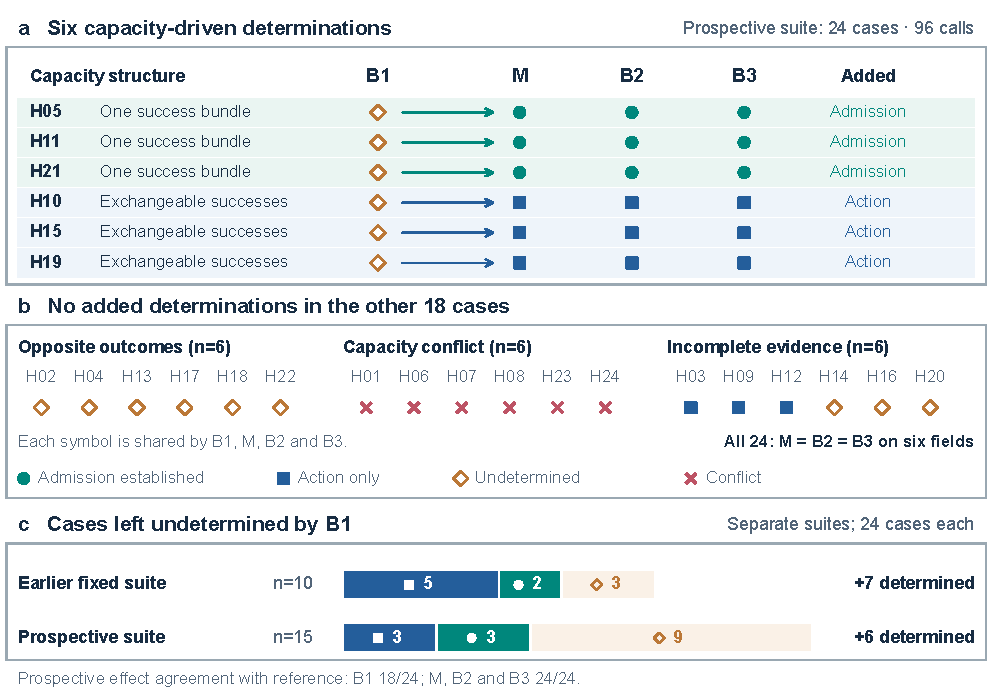
\includegraphics[width=\textwidth]{fig9.pdf}
\caption{Additional verdicts under global capacity constraints. (a) Six capacity-determined cases, split between a single successful bundle and exchangeable successes, with exact baselines. (b) The other 18 prospective instances. (c) Transitions from B1's unresolved verdicts in two separate suites of 24.}\label{fig:9}
\end{figure*}

\subsubsection{Observation completeness and verdict reliability (RQ3)}

Reliability has two requirements: the implementation must answer the model's queries correctly, and observations must justify excluding alternative explanations. We tested the first through finite-domain enumeration, equivalent encodings and process replay. Paired evidence removal, counterexamples to incorrect premises and incomplete archival records tested the second.

\paragraph{Finite-domain checks.} On all 26,880 labeled inputs in the prespecified domain, M agreed field by field with the separately implemented enumeration reference. Each input admitted at most 72 explanations. With the authorization requirement fixed, the six fields covered run status, request processing, execution effect, joint applicability of \textit{must}/\textit{may}, and their two values. A rejection inconsistent with a verified unique source link produced a conflict. If target processing was unobserved, the effect remained unresolved. Four separate inputs had no target record. Complete request records supported a verdict of no successful target action; unconfirmed coverage left the verdict unresolved. Neither Boolean was reported for these four inputs. All 48 pairs of equivalent encodings yielded identical verdicts: 34 pairs produced different normalized views and 14 normalized to the same view. All 720 fresh-process replays reproduced the archived outputs within 10~s each.

\paragraph{Paired removal of observations.} The full and restricted views differed only in explicit request links; both retained the same coverage and capacity assumptions. The four methods agreed on all 18 formal native queries. Removing request coverage made all 18 unresolved: an unobserved initiator could account for the action on actual requests, and the absence of a target could no longer be established for C0. Removing either action coverage or evidence of an initially empty rule set downgraded three admissions to action only (Fig.~\ref{fig:8}b). In the initial cohort, removing request coverage made nine queries unresolved; removing the empty pre-state downgraded three to action only. Source coverage therefore affects which request can be credited with an action, whereas the resource pre-state determines whether the write established new access. The 90 combinations of 18 formal queries and five views are dependent within windows and within queries.

\paragraph{Counterexamples to incorrect premises.} Six controls showed how an unsupported premise can produce a determinate but unjustified verdict. Falsely asserting request coverage excluded an unobserved initiator and changed unresolved to admission established. Falsely asserting action coverage excluded a missing success and changed unresolved to no successful target action. Incorrect capacity or an incorrect explicit link fixed an assignment prematurely, changing unresolved to action only. An incorrectly asserted empty pre-state, or an omitted competing write despite asserted coverage, changed action only to admission established. Each control retained the alternative explanation that the incorrect premise had excluded. These counterexamples show why record completeness, the capacity bound and explicit request links each require independent support.

The fixed suite isolates the contribution of source constraints from that of native observation coverage. On its 24 sealed base instances, replacing explicit assignments with preset same-resource candidates made seven previously determinate effects and one conflict unresolved. Two further variants asserted unverified coverage or lifecycle conditions; both yielded determinate verdicts unsupported by the evidence.

A control using only subsequent HTTP reachability matched B2 on 13/24 effects. It credited four targets with successful actions where exact enumeration found none; three of these targets had been explicitly rejected. Conversely, the control reported only action success in all three cases where exact enumeration established new admission. An HTTP response can therefore both misattribute a success and obscure the difference between a successful write and newly established access.

\paragraph{Resource evidence.} Starting with target success and all other conditions established, removing any one of the seven lifecycle conditions changed admission established to action only, as required by the conjunction in Eq.~\eqref{eq:admit}. The three formal C2 queries provided a native check of the empty pre-state: hiding it left attribution of the successful write intact, but an existing rule could also explain subsequent reachability (Fig.~\ref{fig:8}b). Appendix~E documents the frozen inputs and per-instance witnesses.

\paragraph{Archival observations.} The ablations show how a missing observation changes a verdict. The archived runs illustrate how those gaps arise in recorded evidence. For K02 and K04 the receiver recorded rejections at the flood and replay checks, respectively. Both subsequent HTTP 200 responses were consistent with earlier admission. K03 reached application processing, but its records did not independently establish an empty pre-state. Figure~\ref{fig:10} separates the receiver checkpoint from the independent probe in each of six scenarios.

\begin{figure*}[t]\centering
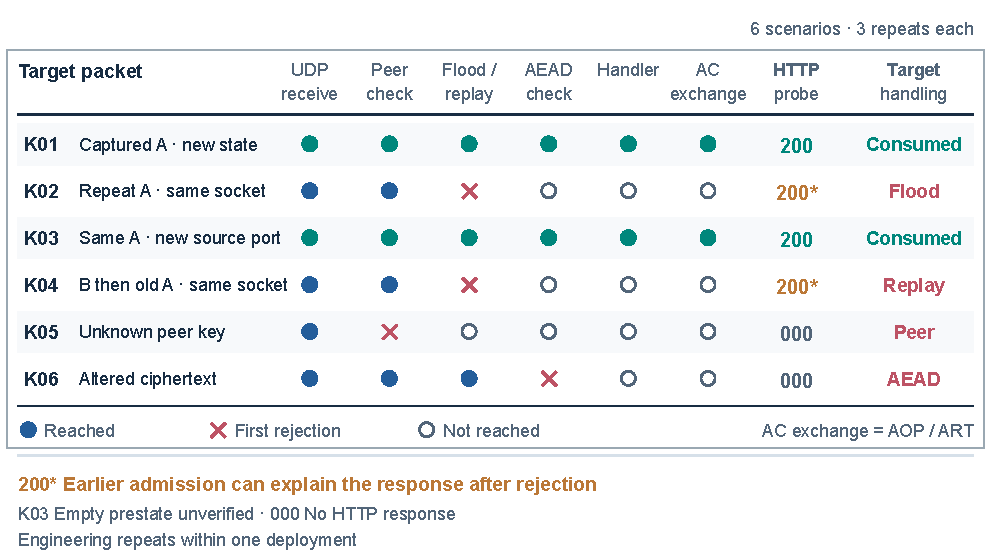
\includegraphics[width=\textwidth]{fig10.pdf}
\caption{Archived KNK receiver checkpoints and independent HTTP probes. Filled and open circles denote reached and unreached stages; a cross marks the first rejection. ``Consumed'' denotes application processing. A prior admission can explain 200*; 000 denotes no HTTP response. Each scenario had three engineering repeats.}\label{fig:10}
\end{figure*}

R02 contained evidence of an empty rule set, a failed external probe while the service was healthy, subsequent application processing, an AC log entry reporting a successful rule addition and a fresh connection that received HTTP 200. It lacked independent post-state rule readback and verified coverage of competing initiators. The R03 records likewise did not establish that the request was freshly generated after expiry: the two observations of packet B referred to the same captured packet, and the distinct packet C in the supplement had already reached application processing. The independent C2 cohort in Section~4.2.1 established request generation after confirmed expiry.

Across 16 incomplete archival inputs, M and B1 agreed: processing and effect remained unresolved for seven DRG inputs; five KNK inputs reached application processing with unresolved effect; and four KNK inputs were explicitly rejected with no successful target action. Authorization remained unresolved in all 16. B2 agreed on the 15 inputs it completed; one reached its enumeration cap (Fig.~\ref{fig:S1}). In receiver-side negative controls, K05 was rejected by the peer check and K06 by authenticated decryption; neither yielded an HTTP response. All scenarios had three repeats on the same deployment; K04 and K05 used corrected valid sequences. Appendix~D gives the cross-interface archival evidence and the policy sources used to distinguish effects from authorization.

\subsubsection{Online evidence collection and offline analysis costs (RQ4)}\label{sec:cost}
We separate the cost of obtaining evidence from the cost of interpreting it. Online, we measure the incremental cost of event logging and packet capture. Offline, we distinguish solver time from the wall-clock cost of a fresh process.

\paragraph{Admission and response latency.} Figure~\ref{fig:11} shows the paired differences within blocks and the distributions across windows. All 80 windows yielded a valid ACK, complete objects, and the expected final rule state. None of the 40 capture windows recorded kernel packet drops. All 40 event-logging windows passed checks on sequence numbers, end records, and native associations. In the order shown in panel~(c), median knock latencies were 10.38, 11.45, 11.49, and 11.44~ms for T0C0, T0C1, T1C0, and T1C1, respectively (20 windows each). Each increment is estimated from the paired differences within blocks.

Figures~\ref{fig:11} and~\ref{fig:12} use the same four contrasts. Events only, Capture only, and Full collection compare T1C0, T0C1, and T1C1, respectively, with T0C0. Events with capture compares T1C1 with T0C1, isolating the increment from event logging when capture is already enabled.

With full collection, the median paired increase in knock latency was 0.620~ms (95\% interval $[0.021,1.613]$~ms). For a 64~B object, the median change in time to first byte was 0.285~ms ($[-0.088,0.561]$~ms). The median paired change in knock latency after enabling event logging was 1.104~ms without capture ($[-0.360,3.587]$~ms) and $-0.177$~ms with capture ($[-0.746,1.465]$~ms). Both intervals include zero, leaving the separate contribution of logging uncertain under these conditions.

\begin{figure*}[t]\centering
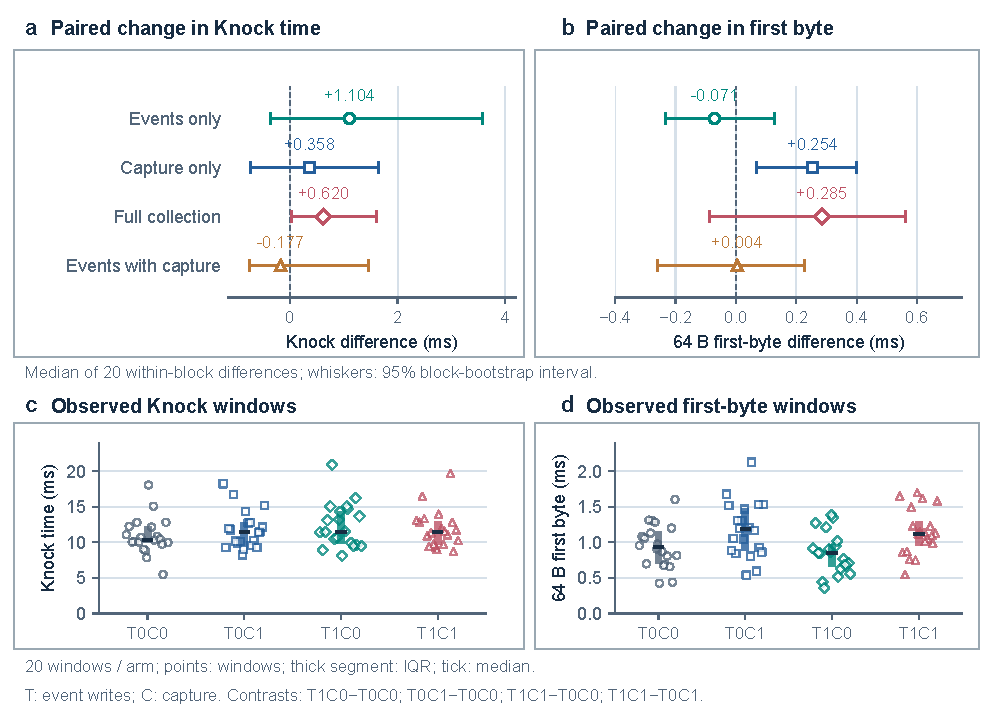
\includegraphics[width=\textwidth]{fig11.pdf}
\caption{Latency under four collection settings on the same build. (a,b) Median of 20 within-block paired differences and 95\% block-resampling intervals. (c,d) Twenty windows per condition; thick segments indicate interquartile ranges and short bars denote medians. T denotes event logging and C denotes capture on both interfaces (0: off; 1: on).}\label{fig:11}
\end{figure*}

\paragraph{Control traffic, object goodput, and storage.} Figure~\ref{fig:12} reports control traffic per admission, application goodput and the storage required for collection. The byte count measures the admission transaction itself. The paired comparisons on the same build quantify the additional cost of collection. In all 40 capture windows, each admission involved one KNK/ACK exchange and one AOP/ART exchange, with no additional target retransmission or cookie exchange. The four UDP payloads totaled 1,538--1,546~B per admission, or 1,650--1,658~B including IPv4 and UDP headers. Individual payloads measured 352~B (KNK), 414--421~B (ACK), 406--409~B (AOP), and 362--364~B (ART). These totals combine Agent--Server control traffic on the virtual Ethernet interface and Server--AC traffic on loopback, excluding startup registration, HTTP, and link-layer overhead. With full collection, median round-trip times measured on the respective interfaces were 8.98~ms for KNK/ACK and 4.77~ms for AOP/ART. The latter exchange occurs during processing of the former, so the two times are reported separately.

\begin{figure*}[t]\centering
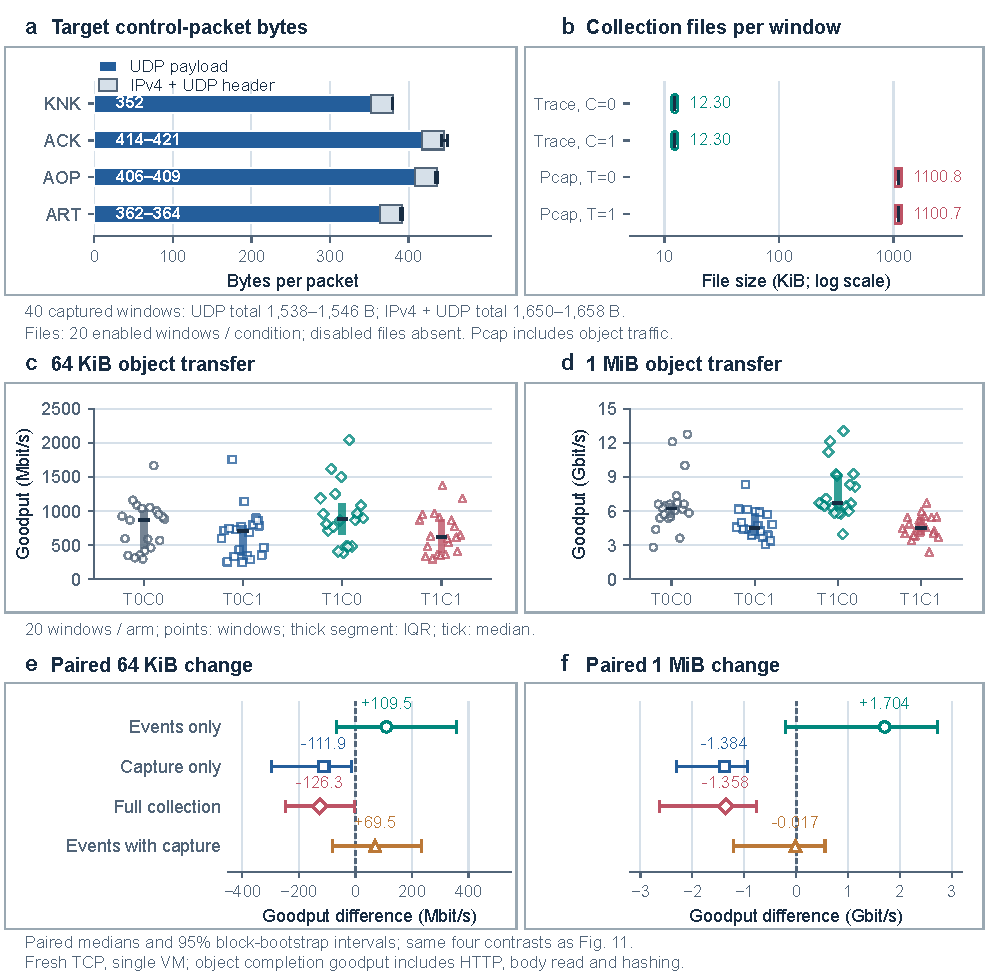
\includegraphics[width=\textwidth]{fig12.pdf}
\caption{Control traffic, collection storage, and object goodput. (a) Median UDP payload and 28~B of headers across 40 windows; ranges inside the bars describe payloads and end marks indicate ranges of total IP lengths. (b) Event and capture file sizes on a logarithmic KiB scale (20 windows per enabled condition). (c,d) Per-window goodput for two object sizes. (e,f) Median paired differences and 95\% resampling intervals across 20 blocks. Settings and contrast order follow Fig.~\ref{fig:11}. Captures include object traffic.}\label{fig:12}
\end{figure*}

For 64~KiB objects, median goodput was 876.2~Mbit/s under T0C0 and 627.0~Mbit/s under T1C1. For 1~MiB objects, the corresponding medians were 6.232 and 4.504~Gbit/s.

For the two object sizes, the paired goodput differences under full collection had medians of $-126.3$~Mbit/s and $-1.358$~Gbit/s. The respective intervals were $[-246.0, -3.3]$ and $[-2.626, -0.767]$ in the same units. For the 1~MiB object, capture alone produced a median paired difference of $-1.384$~Gbit/s. Its interval was $[-2.313, -0.931]$~Gbit/s. Adding event logging to capture produced a median paired difference of $-0.017$~Gbit/s, with an interval from $-1.215$ to $0.555$~Gbit/s.

Under full collection, median storage per window was 12.30~KiB for events and 1.075~MiB for the two capture files combined. Those files include control, probe, and object traffic. Panel~(a) reports the control transaction alone.

\paragraph{Offline analysis.} Global queries test feasibility without enumerating explanations. Their cost depends on the candidate graph, whereas enumeration also depends on how many missing sources, outcomes, and actions the observations admit. In archival input R03-C, each of eight action bundles had only one visible candidate but could also have an external origin. Each outcome was unknown, and a target action might have gone unrecorded. These alternatives yielded $2^8\times2^8\times2=131{,}072$ explanations; B2 reached its cap of 100,000. Counting visible candidates alone therefore understates enumeration cost.

Section~\ref{sec:correctness} gives the query and complexity bounds. Table~\ref{tab:8} summarizes observed workloads. Fixed-regression base graphs contained at most four requests, four action bundles, and 11 candidate edges; B2 enumerated at most 12 compatible explanations. Prospective sealed graphs contained four to six requests, two to six bundles, and four to 24 visible edges. M ran one to seven checks per instance (median three); B2 enumerated zero to 38 compatible explanations, with none on the six conflicting inputs. All 96 first-round calls finished within budget. The longest process took 159.54~ms, including startup and dependency loading.

\begin{table*}[t]\centering
\caption{Computation on archival replay and the first prospective synthetic evaluation.}\label{tab:8}
\begin{tabularx}{\textwidth}{@{}lXX@{}}\toprule
Check & Unit & Result \\ \midrule
Equivalent encodings & 48 pairs from development and sealed base instances & All 48 pairs agreed; 34 changed the normalized solver view. \\
Process replay & 672 synthetic calls and 48 calls on historical evidence & All 720 results matched the archive. \\
Historical replay budget & 10~s per call; B2 capped at 100,000 compatible explanations & No process timed out; one historical input reached the enumeration cap. \\
Prospective first round & 24 instances, one call per method on each & All 96 calls completed within budget; each method returned 18 regular results and six conflicts. \\
Prospective workload & Implementation counters per instance & M: 1--7 feasibility checks; B2: 0--38 compatible explanations. \\ \bottomrule
\end{tabularx}
\end{table*}

Figure~\ref{fig:13} reports solver time, preparation time and the duration of each fresh-process call. All 480 fresh-process calls completed within budget; all six output fields matched the first round. Each point is the mean over 24 inputs for one method in one block.

\begin{figure*}[t]\centering
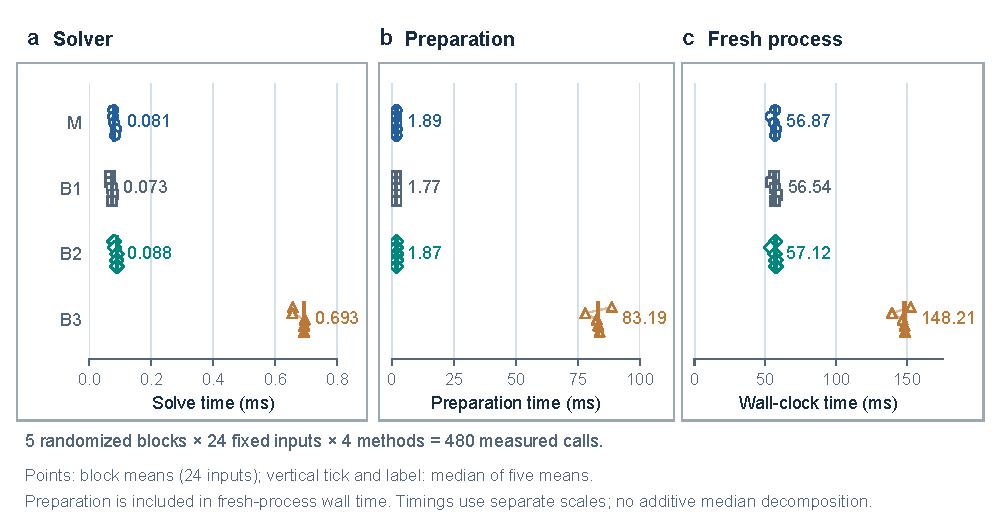
\includegraphics[width=\textwidth]{fig13.pdf}
\caption{Computation on small sealed graphs. (a) Solver time. (b) Preparation time. (c) Fresh-process wall time, including preparation. Each point is the mean over 24 instances in one block; vertical marks indicate the median of the five block means. Axis scales differ across panels.}\label{fig:13}
\end{figure*}

For M, B1, B2, and B3, the medians of five block means were, respectively, 0.081, 0.073, 0.088, and 0.693~ms for solving and 56.87, 56.54, 57.12, and 148.21~ms for the full process. Preparation took 1.89, 1.77, 1.87, and 83.19~ms, respectively; peak resident memory was 27.28, 27.27, 27.33, and 44.22~MiB. B3 uses the NetworkX minimum-cost-flow interface. Its 83.19~ms preparation time combines method-module loading, input reading and parsing, and process checks. On these 24 small sealed graphs, M matched the exact reference with submillisecond solver time. Most fresh-process wall time was spent outside the solver.
